\documentclass[12pt,twoside]{report}    

\usepackage[phd]{otagothesis}   %% Use Otago page layout
\usepackage{natbib} 		%% author/year format in round brackets
\usepackage{graphicx}           %% jpg, gif, tiff, and pdf graphics
\usepackage{moreverb}           %% Verbatim Code Listings
\usepackage{amsmath}		%% More math commands
\usepackage{amssymb}		%% More math commands
\usepackage{amsthm}		%% More math commands
\usepackage{mathrsfs}		%% More math commands
\usepackage{color}		%% Handling colors
\usepackage{enumerate}          %% Fancy enumeration lists

%%%%%%%%%%%%%%%%%%%%%%%%%%%%% New commands 

\newcommand{\BigO}[1]{{\rm O}\left(#1\right)}
\newcommand{\expo}{\,\mathrm{e}}
\newcommand{\cvar}{\,\mathrm{i}}
\newcommand{\besseli}{\mathrm{I}}
\newcommand{\besselk}{\mathrm{K}}
\newcommand{\bessely}{\mathrm{Y}}
\newcommand{\besselj}{\mathrm{J}}
\newcommand{\eg}{e.g.\ }
\newcommand{\elemvec}[2]{\big[#1\big]_{#2}}
\newcommand{\ud}[1]{\,\mathrm{d}#1}
\newcommand{\hPhi}{\widehat{\Phi}}
\newcommand{\diag}[1]{\text{diag}\left\{#1\right\}}
\renewcommand{\Re}{\operatorname{Re}}
\renewcommand{\Im}{\operatorname{Im}}


\newcommand{\TODO}[1]{\textcolor{red}{\bf{[#1]}}}

\newtheorem{lemma}{Lemma}
\newtheorem{theorem}{Theorem}
%%%%%%%%%%%%%%%%%%%%%%%%%%% Front page info 

\title{Inference and Characterization of Planar Trajectories}
\author{Jerome}
%\date{15 June 2012}

%%%%%%%%%%%%%%%%%%%%%%%%%%%%%% Extra info 

%\fullname{Jerome}
%\department{Department of Mathematics and Statistics}
%\dob{3 January 1985} %% date-of-birth
%\address{42A Cargill st, Dunedin, New Zealand}



%% Uncomment to just print up a few chapters.
%%
%\includeonly{}

\begin{document}


%% Put in titlepage and contents, etc...
\frontstuff

%% Set to one-and-a-half line-spacing
\linespread{1.3} \normalsize

%% Chapters

\setcounter{chapter}{1}
\section{Introduction}
%GPS units of a tractor working on an orchard could provide some information, including position, velocity, acceleration, etc, with which an orchardist is able to follow the trajectory and motion patterns of tractors. 

%The observed position data set $y_i$ always comes with some errors $\varepsilon_i$, which are assumed independent Gaussian distribution with variance $\sigma_n^2$. A popular method for finding $f(x)$ that fits these data is to augment/replace the vector of inputs $\mathbf{X}$ with additional variables, which are transformations of $\mathbf{X}$, and then use linear models in this new space of derived input features.\cite{esl2009}

Denote by $h_m(t):\mathbb{R}^p \mapsto \mathbb{R}$ the $m$th transformation of $\mathbf{T}$, $m =1, \cdots ,M$. \TODO{what is $\mathbf{T}$?} We then model
\begin{equation*}
f(t) =\sum_{m=1}^{M}\beta_mh_m(t).
\end{equation*}
\TODO{best to number all your equations; someone will want to reference them} a linear basis expansion in $\mathbf{T}$, where $h_m(t)$ are called basis functions and $\beta_m$ are coefficients.

Among all functions $f(t)$ with two continuous derivatives fitting these observed data, there is only one unique $f(t)$, \TODO{proof???} which can be found by minimizing the following penalized residual sum of squares, returning the smallest errors,
\begin{equation}\label{mse}
\text{MSE}(f,\lambda)=\frac{1}{n}\sum_{i=1}^n(f(t_i)-y_i)^2+\lambda \int_{0}^{1}(f''(t))^2dt
\end{equation}
where $\lambda$ is a fixed smoothing parameter, $(t_i,y_i)$, $i=1, \cdots, n$ are observed data and $0 \leq t_1< t_2 < \cdots <t_n \leq 1$. In equation (\ref{mse}),  the smoothing parameter $\lambda$ controls the smoothness of function $f(t)$,
\begin{align*}
\begin{cases}
\lambda = 0 : & \mbox{$f$ can be any function that interpolates the data,}\\
\lambda = \infty: & \mbox{the simple least squares line fit since no second derivative can be tolerated.}\\
\end{cases}
\end{align*}

In our case, the velocity data set $v_i$ with some independent Gaussian distributed errors $\varepsilon_i \sim N(0, \frac{\sigma_n^2}{\gamma})$ are used to estimate $f(t)$ as well. The velocity information  is incorporated into MSE  equation (\ref{mse}) by the addition of velocity term $(f'(t_i)-v_i)^2$. Then it becomes 
\begin{equation}\label{mse2}
\text{MSE}(f,\lambda,\gamma)=\frac{1}{n}\sum_{i=1}^n(f(t_i)-y_i)^2+\frac{\gamma}{n} \sum_{i=1}^n(f'(t_i)-v_i)^2+\lambda \int_{0}^{1}(f''(t))^2dt.
\end{equation}

In the model $y=f(t)+\varepsilon$, it is reasonable to assume that the observed data $y_i$ is Gaussian distribution with mean $f(t_i)$ and variance $\sigma_n^2$. In a similar way, the velocity is estimated as  $v=f'(t)+\frac{\varepsilon}{\gamma}$, where $v_i$ is Gaussian distribution with mean $f'(t_i)$ and variance $\frac{\sigma_n^2}{\gamma}$. Then the joint distribution of $\mathbf{Y},\mathbf{V},f(t)$ and $f'(t)$ is normal with zero mean and a covariance matrix, which can be estimated through Gaussian Process Regression.

\section{Gaussian Process Regression}

A Gaussian Process (GP) is a collection of random variables, any finite number of which have a joint Gaussian distribution, \cite{b_gpml}.

A GP is fully defined by its mean $m(t)$ and covariance $K(s,t)$ functions as
\begin{align*}
m(t)&=\mathbb{E}[f(t)] \\
K(s,t)&=\mathbb{E}[(f(s)-m(s)) (f(t)-m(t))],
\end{align*}
where $s$ and $t$ are two variables, and a function $f$ distributed as such is denoted in form of
\begin{equation}
f \sim GP(m(t),K(s,t)).
\end{equation}
Usually the mean function is assumed to be zero everywhere. 

Given a set of input variables $\mathbf{T}$ for function $f(t)$ and the output $\mathbf{Y}=f(\mathbf{T})+\varepsilon$ with independent identically distributed Gaussian noise $\varepsilon$ with variance $\sigma_n^2$,  we can use the above definition to predict the value of the function $f_*=f(t_*)$ at a particular input $t_*$. As the noisy observations becoming
\begin{align*}
\text{cov}(y_p,y_q) = K(t_p,t_q)+\sigma_n^2 \delta_{pq}
\end{align*}
where $\delta_{pq}$ is a Kronecker delta which is one iff $p=q$ and zero otherwise, the joint distribution of the observed outputs $\mathbf{Y}$ and the estimated output $f_*$ according to prior is
\begin{equation}
\left[ \begin{matrix}
\mathbf{Y}\\
f_*
\end{matrix} \right] \sim N \left(  
0,\left[   \begin{matrix}
K(\mathbf{T},\mathbf{T}) +\sigma_n^2I& K(\mathbf{T},t_*) \\
K(t_*,\mathbf{T}) & K(t_*,t_*)
\end{matrix}  \right] 
\right).
\end{equation}
The posterior distribution over the predicted value is obtained by conditioning on the observed data \TODO{cov goes to var here???}
\begin{equation}
f_* | \mathbf{Y},\mathbf{T},t_* \sim N(\bar{f_*},\text{cov}(f_*))
\end{equation}
where 
\begin{align*}
\bar{f_*}&=\mathbb{E}[f_* | \mathbf{Y},\mathbf{T},t_* ]=K(t_*,\mathbf{T})[K(\mathbf{T},\mathbf{T})+\sigma_n^2I]^{-1}\mathbf{Y},\\
\text{cov}(f_*)&=K(t_*,t_*)-K(t_*,\mathbf{T})[K(\mathbf{T},\mathbf{T})+\sigma_n^2I]^{-1}K(\mathbf{T},t_*).
\end{align*}

We now add velocity information $\mathbf{V}$. It is assumed that the velocity $\mathbf{V}=f'(\mathbf{T})+\frac{\varepsilon}{\sqrt{\gamma}}$, where $\varepsilon$ is as the same \TODO{you mean same in distribution. explain more clearly. also no correlation} as that in $\mathbf{Y}$. 

It is expected that a position point $y_i$ and velocity point $v_i$ are all effected by other points $\mathbf{Y}$ and $\mathbf{V}$. So the covariance matrix for $\mathbf{Y}$ and $\mathbf{V}$ is
\begin{equation}\label{covYV}
\Sigma(\mathbf{Y},\mathbf{V}) = 
\left[
\begin{matrix}
\text{cov}(\mathbf{Y},\mathbf{Y}) & \text{cov}(\mathbf{Y},\mathbf{V}) \\
\text{cov}(\mathbf{V},\mathbf{Y}) & \text{cov}(\mathbf{V},\mathbf{V}) 
\end{matrix}\right],
\end{equation}
where obviously $\text{cov}(\mathbf{Y},\mathbf{V}) =\text{cov}(\mathbf{V},\mathbf{Y})$. Then the joint distribution  is 
\begin{equation*}
\left[
\begin{matrix}
\mathbf{Y}\\
\mathbf{V}
\end{matrix}
\right] \sim N(\mu_{y,v},\Sigma_{y,v}).
\end{equation*}
Define $f_*$ and $f'_*$ the estimated position and velocity values at point $t_*$. From equation (\ref{covYV}) and using similar idea, it is easily to get the covariance matrices 
\begin{align*}
\Sigma(f_*,\mathbf{V}) = 
\left[
\begin{matrix}
\text{cov}(f_*,f_*) & \text{cov}(f_*,\mathbf{V}) \\
\text{cov}(\mathbf{V},f_*) & \text{cov}(\mathbf{V},\mathbf{V}) 
\end{matrix}\right],
\Sigma(\mathbf{Y},f'_*) = 
\left[
\begin{matrix}
\text{cov}(\mathbf{Y},\mathbf{Y}) & \text{cov}(\mathbf{Y},f'_*) \\
\text{cov}(f'_*,\mathbf{Y}) & \text{cov}(f'_*,f'_*) 
\end{matrix}\right],
\end{align*}
\begin{align*}
\Sigma(f_*,f'_*) = 
\left[
\begin{matrix}
\text{cov}(f_*,f_*) & \text{cov}(f_*,f'_*) \\
\text{cov}(f'_*,f_*) & \text{cov}(f'_*,f'_*) 
\end{matrix}\right],
\end{align*}

\TODO{will need to give the form of these covariances at some point. in an appendix? i think you need discussion of how $f'$ is related to $f$ for a GP}



\section{A Reproducing Kernel in Space $\mathbb{H}$}

$N_1(t), \cdots, N_n(t)$ denote $n$ basis functions in space $\mathbb{H}$. For any continuous function $f \in \mathbb{H}$, it is a combination of these basis functions
\begin{equation*}
f(t)=\sum_{i=1}^{n} \alpha_iN_i(t),
\end{equation*}
where $\alpha_i (i=1, \cdots, n)$ are coefficients. With an inner product \TODO{use \textbackslash langle for $<$,  \textbackslash rangle for $>$}
\begin{equation}
<f,g>= <\sum_{i=1}^{n} \alpha_iN_i(t), \sum_{i=1}^{n} \beta_iN_i(t)>=\sum_{i=1}^{n} \alpha_i \beta_i, 
\end{equation}
it can be shown that the representer of evaluation $[s](\cdot)$ is
\begin{equation}
R_s(t) = \sum_{i=1}^{n} N_i(s)N_i(t),
\end{equation}
Then we can prove that the space $\mathbb{H}$ is a Reproducing Kernel Hilbert Space. In fact,
\begin{align*}
<f(t), R(s,t)>=<\sum_{i=1}^{n} \alpha_iN_i(t),  \sum_{i=1}^{n} N_i(s)N_i(t)>=\sum_{i=1}^{n}\alpha_iN_i(s)=f(t).
\end{align*}
The term $R(s,t)=R_s(t)$ is called the reproducing kernel function.


We now introduce a new notation $\dot{R}(s,t)$ in the following and use it to find the covariance matrix $\Sigma$ of the joint distribution of $\mathbf{Y}, \mathbf{V}, f$ and $f'$.

Define $\dot{R}(s,t)$ and $R'(s,t)$ are the first partial derivative of $R(s,t)$ with respect to the first  and second argument respectively
\begin{align} \label{dotr}
\dot{R}(s,t)=\frac{\partial R(s,t)}{\partial s}=\sum_{i=1}^{n} \frac{dN_i(s)}{ds}N_i(t)=\sum_{i=1}^{n} N'_i(s)N_i(t),\\
\label{dotr2}
 R'(s,t)=\frac{\partial R(s,t)}{\partial t}=\sum_{i=1}^{n} N_i(s)\frac{dN_i(t)}{dt}=\sum_{i=1}^{n} N_i(s)N'_i(t),
\end{align}
Then $\dot{R}'(s,t)$ is the second partial derivative of $R(s,t)$ with respect to both arguments
\begin{equation*}
\dot{R}'(s,t)=\frac{\partial^2 R(s,t)}{\partial s \partial t}=\sum_{i=1}^{n} \frac{dN_i(s)}{ds}\frac{dN_i(t)}{dt}=\sum_{i=1}^{n} N'_i(s)N'_i(t).
\end{equation*}
It is easily to prove that $\dot{R}(s,t)=R'(t,s)$ and
\begin{align*}
<f(t), R'(s,t)> = <\sum \alpha_i N_i(t), \sum N_i(s)N'_i(t)> =   \sum \alpha_i N_i(s) =f(t),\\
<f'(t), \dot{R}(s,t)> = <\sum \alpha_i N_i(t), \sum N'_i(s)N_i(t)> =   \sum \alpha_i N'_i(s) =f'(t),\\
<f'(t), \dot{R}'(s,t)> = <\sum \alpha_i N_i(t), \sum N'_i(s)N'_i(t)> =   \sum \alpha_i N'_i(s) =f'(t),\\
<\dot{R}(s,t),f(t)> = <\sum N'_i(s)N_i(t), \sum \alpha_i N_i(t), > =   \sum \alpha_i N'_i(s) =f'(t),\\
<R'(s,t),f'(t)> = <\sum N_i(s)N_i'(t), \sum \alpha_i N'_i(t)> =   \sum \alpha_i N_i(s) =f(t).
\end{align*}

Given the sample points $t_i, i=1, \cdots, n$ and noting that the space
\begin{equation*}
\mathbb{A}=\{f: f=\sum_{i=1}^{n}\alpha_iR(t_i,\cdot) \} 
\end{equation*}
is one linear subspace of $\mathbb{H}$. Then $f \in \mathbb{H}$ can be written as
\begin{equation}\label{etaeq}
f(t)=\sum_{i=1}^{n}c_iR(t_i,t)+\rho(t)
\end{equation}
where $c_i$ are coefficients, $\rho(t) \in \mathbb{H} \ominus \mathbb{A} $, and 
\begin{equation}\label{etaeq2}
f'(t)=\sum_{i=1}^{n}c_iR'(t_i,t)+\rho'(t).
\end{equation}

The equation (\ref{mse2}) can be written as
\begin{align*}
\frac{1}{n}\sum_{i=1}^n (y_i -\sum_{j=1}^{n}c_jR(t_j,t_i) -\rho(t_i))^2+
\frac{\gamma}{n}\sum_{i=1}^n (v_i -\sum_{j=1}^{n}c_jR'(t_j,t_i) -\rho'(t_i))^2 \\
+\lambda \int_{t_1}^{t_n} (\sum_{j=1}^{n}c_jR''(t_j,t)+\rho''(t))^2dt
\end{align*}
As $\dot{R}(t_i,\cdot) = \sum_{j=1}^{n}N_j'(t_i)N_j(t) \in \mathbb{A}$, then by orthogonality and property of reproducing kernel functions, $\rho(t_i)=<R(t_i,\cdot),\rho>=0$, %$\rho(t_i) =<\rho,R'(\cdot,t_i)>=<\dot{R}(t_i,\cdot),\rho>=0$, 
and $\rho'(t_i)=<\rho,R'(t_i,\cdot)>=<\dot{R}(t_i,\cdot),\rho>=0$, where $i=1,\cdots,n$. 

Denoting by $Q$ the $n \times n$ matrix with the $(i,j)$th entry $R(t_i,t_j)$, by $P$ the $n \times n$ matrix with the $(i,j)$th entry $\dot{R}'(t_i,t_j)$ the equation (\ref{mse2}) can be written as
\begin{equation}\label{matrixeq}
(\mathbf{Y}-Q\mathbf{c})^T(\mathbf{Y}-Q\mathbf{c})+\gamma (\mathbf{V}-P\mathbf{c})^T(\mathbf{V}- P\mathbf{c})+n\lambda \Omega+\lambda(\rho,\rho).
\end{equation}
Note that $\rho$ only appears in the third term in $(\ref{matrixeq})$, which is minimized at $\rho=0$. Hence, a polynomial smoothing spline resides in the space $\mathbb{A} $ of finite dimension. Then the solution could be computed via minimization of term in $(\ref{matrixeq})$ with respect to $\mathbf{c}$, \cite{gubook}.

\section{Covariance Matrix and Posterior Mean}

Consider $f$ and $f'$ in $\mathbb{H}$, having Gaussian priors with zero mean and covariance functions
\begin{align*}
\text{cov}(f(s),f(t))&=\tau^2 R(s,t)+\sigma_n^2\Lambda\\
\text{cov}(f(s),f'(t))&=\tau^2 R'(s,t)+\frac{\sigma_n^2}{\sqrt{\gamma}}\Lambda\\
\text{cov}(f'(s),f(t))&=\tau^2 \dot{R}(s,t)+\frac{\sigma_n^2}{\sqrt{\gamma}}\Lambda\\
\text{cov}(f'(s),f'(t))&=\tau^2 \dot{R}'(s,t)+\frac{\sigma_n^2}{\gamma}\Lambda
\end{align*}
where $\Lambda$ is the correlation matrix \TODO{where does $\Lambda$ come from?}. Observing $y_i \sim N(f(t_i),\sigma_n^2)$ and $v_i \sim N(f'(t_i),\frac{\sigma_n^2}{\gamma})$, the joint distribution of $\mathbf{Y}, \mathbf{V}, f(t)$ and $f'(t)$ is normal with zero mean and covariance matrix
\begin{align*}
\text{cov}(\mathbf{Y},\mathbf{V},f,f') &= 
\left[ \begin{matrix}
\tau^2R(t_i,t_j)+\sigma_n^2\Lambda & \tau^2R'(t_i,t_j)+\frac{\sigma_n^2}{\sqrt{\gamma}}\Lambda & \tau^2R(t_i,t)& \tau^2R'(t_i,t) \\
\tau^2 \dot{R}(t_i,t_j)+\frac{\sigma_n^2}{\sqrt{\gamma}}\Lambda & \tau^2 \dot{R}'(t_i,t_j)+\frac{\sigma_n^2}{\gamma}\Lambda & \tau^2 \dot{R}(t_i,t)& \tau^2\dot{R}'(t_i,t)  \\
\tau^2R^T(t_i,t) & \tau^2\dot{R}^T(t_i,t) & \tau^2R(t,t)& \tau^2\dot{R}(t,t) \\
 \tau^2R'^T(t_i,t)& \tau^2\dot{R}'^T(t_i,t)& \tau^2R'(t,t)& \tau^2\dot{R}'(t,t)  \\
\end{matrix} \right] \\
&=
\left[ \begin{matrix}
\tau^2Q+\sigma_n^2\Lambda & \tau^2 O+\frac{\sigma_n^2}{\sqrt{\gamma}}\Lambda & \tau^2\xi & \tau^2\xi' \\
\tau^2 O+\frac{\sigma_n^2}{\sqrt{\gamma}}\Lambda & \tau^2 P+\frac{\sigma_n^2}{\gamma}\Lambda & \tau^2 \dot{\xi}& \tau^2\dot{\xi}' \\
\tau^2\xi^T & \tau^2\dot{\xi}^T & \tau^2R(t,t)& \tau^2\dot{R}(t,t) \\
 \tau^2\xi'^T& \tau^2\dot{\xi}'^T& \tau^2R'(t,t)& \tau^2\dot{R}'(t,t)  \\
\end{matrix} \right]
\end{align*}
where $\{Q\}_{ij}$ is the matrix with elements $R(t_i,t_j)$,  $\{O\}_{ij}$ is the matrix with elements $\dot{R}(t_i,t_j)=R'(t_j,t_i)$,  $\{P\}_{ij}$ is the matrix with elements $\dot{R}'(t_i,t_j)$, $\xi$ is a $n \times 1$ matrix with $i$th elements $R(x_i,x)$, and $\dot{\xi}$ is a $n \times 1$ matrix with $i$th elements $\dot{R}(x_i,x)$. Then
\begin{align*}
E\left[ \begin{matrix}
f \\
f'
\end{matrix} | \begin{matrix}
\mathbf{Y} \\
\mathbf{V}
\end{matrix}\right] &= 
\left[ \begin{matrix}
\xi^T& \dot{\xi}^T \\
\xi'^T & \dot{\xi}'^T 
\end{matrix} \right] 
\left[ \begin{matrix}
Q+n\lambda \Lambda & O+\frac{n\lambda}{\sqrt{\gamma}}\Lambda\\
 O+\frac{n\lambda}{\sqrt{\gamma}}\Lambda &  P+\frac{n\lambda}{\gamma}\Lambda
\end{matrix} \right] ^{-1}
\left[ 
\begin{matrix}
\mathbf{Y} \\
\gamma \mathbf{V}
\end{matrix} \right] \\
&\triangleq
\left[ \begin{matrix}
\xi^T& \dot{\xi}^T \\
\xi'^T & \dot{\xi}'^T 
\end{matrix} \right] 
\left[ \begin{matrix}
A & B\\
C & D
\end{matrix} \right]
\left[ 
\begin{matrix}
\mathbf{Y} \\
\gamma \mathbf{V}
\end{matrix} \right] \\
&=
\left[ \begin{matrix}
\xi^T(A\mathbf{Y}+B\gamma \mathbf{V})+ \dot{\xi}^T(C\mathbf{Y}+D\gamma \mathbf{V}) \\
\xi'^T(A\mathbf{Y}+B\gamma \mathbf{V})+ \dot{\xi}'^T(C\mathbf{Y}+D\gamma \mathbf{V}) 
\end{matrix} \right] 
\end{align*}
where $n\lambda = \sigma_n^2 / \tau^2$. The posterior mean $E(f | \mathbf{Y},\mathbf{V})$ is of the form $\xi^T \mathbf{c}+\dot{\xi}^T\mathbf{d}$ and $E(f' | \mathbf{Y},\mathbf{V})$ is of the form $\xi'^T \mathbf{c}+\dot{\xi}'^T\mathbf{d}$, with the same coefficients given by
\begin{align*}
\mathbf{c}&=A\mathbf{Y}+B\gamma \mathbf{V}\\
\mathbf{d}&=C\mathbf{Y}+D\gamma \mathbf{V} 
\end{align*}



\section{A 1-D Gaussian Process Spline Construction}
Trajectories are represented by a series of 2D position points $(x_t,y_t)$ and velocity points $(u_t,v_t)$ corresponding to measurements taken at discrete time steps $t$, where $x_t$ and $u_t$ represented longitude, $y_t$ and $v_t$ represented latitude position and velocity respectively \cite{ellis2009}. For now, we just focus on the problem of fitting trajectories in 1 Dimension situation. 

For any $t \in [t_1,t_n]$, we wish to estimate the latitude position $y(t)$ and velocity $v(t)$ with model
\begin{align*}
y(t)&=f(t)+\varepsilon,\\
v(t)&=f'(t)+\frac{\varepsilon}{\gamma},
\end{align*}
where $\varepsilon$ is zero-mean Gaussian noise. A Gaussian process prior over $f \sim GP(m(t),K(s,t))$ leading to the approximate estimation model
\begin{equation}\label{xvgp}
p(y_t,v_t | \mathbf{Y}, \mathbf{V}) \sim N(GP_\mu (\mathbf{Y}, \mathbf{V}), GP_\Sigma (\mathbf{Y}, \mathbf{V})).
\end{equation} 

\subsection{Tractor Spline}

Suppose we have observed data set $t_1, \cdots, t_n$ satisfying $t_1<t_2<\cdots<t_n$. The function $f(t)$ defined on this interval $[t_1,t_n]$ is called tractor spline, if on each interval $(t_i,t_{i+1})$, $i=2,\cdots,n-2$, $f(t)$ is a cubic polynomial, but on interval $(t_1,t_2)$ and $(t_{n-1},t_n)$ can be a linear function; $f(t)$ fits together at each point $t_i$ in such a way that $f(t)$ itself and its first and second derivatives are continuous at each $t_i$.  

Define some basis functions on interval $[t_1,t_n]$. On an arbitrary interval $[t_i,t_{i+1}]$, we have Hermite Spline basis functions as following
\begin{align*}
&h_{00}^{(i)}(t)=
\begin{cases}
2(\frac{t-t_{i}}{t_{i+1}-t_{i}})^3-3(\frac{t-t_{i}}{t_{i+1}-t_{i}})^2+1, & t_i\leq t \leq t_{i+1} \\ 
0 & otherwise
\end{cases}, \\
&h_{10}^{(i)}(t)=\begin{cases}
\frac{(t-t_{i})^3}{(t_{i+1}-t_{i})^2}-2\frac{(t-t_{i})^2}{t_{i+1}-t_{i}}+(t-t_{i}), & t_i\leq t \leq t_{i+1} \\ 
0 &  otherwise
\end{cases},\\
&h_{01}^{(i)}(t)=
\begin{cases}
-2(\frac{t-t_i}{t_{i+1}-t_i})^3+3(\frac{t-t_i}{t_{i+1}-t_i})^2, & t_i\leq t \leq t_{i+1} \\ 
0 &  otherwise
\end{cases},\\
&h_{11}^{(i)}(t)=\begin{cases}
\frac{(t-t_i)^3}{(t_{i+1}-t_i)^2}-\frac{(t-t_i)^2}{t_{i+1}-t_i}, & t_i\leq t \leq t_{i+1} \\ 
0 &  otherwise
\end{cases}.
\end{align*}
 Define $N_1 = h^{(1)}_{00}$, $N_2 = h^{(1)}_{10}$, $N_{2n-1} = h_{01}^{(n)}$, $N_{2n} = h_{11}^{(n)}$. For all $k=1,2,\ldots,n-2$ define $N_{2k+1}$ by
\[N_{2k+1}(t) = \begin{cases} h_{01}^{(k)}+h_{00}^{(k+1)} & t \neq t_{k+1} \\ 1 & t = t_{k+1}.\end{cases}\]
and $N_{2k+2} = h_{11}^{(k)}+h_{10}^{(k+1)}$.

We now prove that $N_1, N_2, \cdots, N_{2n}$ are linear independent. 
\begin{lemma}\cite{peng1983}
Functions $x_1(t),x_2(t),\cdots,x_n(t)$ on interval $[a,b]$, if they are linear dependent, the necessary and sufficient condition is for any $c_1,c_2,\cdots,c_n \in [a,b]$, the determinant $D(c_1,c_2,\cdots,c_n)=0$; if they are linear independent, the necessary and sufficient condition is that there exist $c_1,c_2,\cdots,c_n \in [a,b]$, so that the determinant $D(c_1,c_2,\cdots,c_n) \neq 0$, where 
\begin{equation*}
D(c_1,c_2,\cdots,c_n)=
\begin{vmatrix}
x_1(c_1) & x_1(c_2) & \cdots& x_1(c_n)\\
x_2(c_1) & x_2(c_2)& \cdots & x_2(c_n)\\
 \vdots  &  \vdots  & \ddots  & \vdots  \\  
x_n(c_1) & x_n(c_2) & \cdots & x_n(c_n)\\
\end{vmatrix}
\end{equation*}
\end{lemma}


\begin{theorem}
The functions $N_1,\ldots,N_{2n}$ provide a basis for the set of functions on $[t_1,t_n]$  which are continuous, have continuous first derivatives and which are 
cubic on each open interval $(t_i,t_{i+1})$.
\end{theorem}
\begin{proof}
It is obviously that every basis functions are continuous on subinterval $[t_k,t_{k+1}]$. We firstly prove that these basis functions are independent. 

We have $2n$ basis functions and $n$ knots. Then choose $t_1, \frac{t_1+t_2}{2}, t_2, \frac{t_2+t_3}{2}, \cdots, t_{n-1}, \frac{t_{n-1}+t_n}{3}, \frac{2(t_{n-1}+t_n)}{3}, t_n$ as new $2n$ knots, and denoted by $c_1,c_2,\cdots,c_{2n}$. Then the determinant is
\begin{equation}\label{matrixD}
D(c_1,c_2,\cdots,c_{2n})=
\begin{vmatrix}
N_1(c_1) & N_1(c_2) & \cdots& N_1(c_{2n})\\
N_2(c_1) & N_2(c_2)& \cdots & N_2(c_{2n})\\
 \vdots  &  \vdots  & \ddots  & \vdots  \\  
N_{2n}(c_1) & N_{2n}(c_2) & \cdots & N_{2n}(c_{2n})\\
\end{vmatrix}
=
\begin{vmatrix}
1 & a_{12} & 0 & 0 & \cdots& 0 & 0 \\
0 & a_{22} & 0 & 0 & \cdots& 0 & 0\\
0 & a_{32} & 1 & a_{34} & \cdots& 0 & 0\\
 \vdots  &  \vdots  &  \vdots &  \vdots & \ddots  & \vdots   &  \vdots\\  
0 & 0 & 0 & 0 & \cdots& a_{2n-1,2n-1} & 1\\
0 & 0 & 0 & 0 & \cdots& a_{2n,2n-1} & 0 \\
\end{vmatrix},
\end{equation}
where $D(c_1,c_2,\cdots,c_{2n})=\begin{cases}
N_1(t_1)=1 \\
N_1(\frac{t_1+t_2}{2})=a_{12} \\
N_2(t_1)=0 \\
N_2(\frac{t_1+t_2}{2})=a_{22} \\
N_{2k+1}(\frac{t_k+t_{k+1}}{2})=a_{2k+1,2k} & k=1,2,\cdots,2n \\ 
N_{2k+1}(t_{k+1})=1 & k=1,2,\cdots,2n \\ 
N_{2k+1}(\frac{t_{k+1}+t_{k+2}}{2})=a_{2k+1,2k+2} & k=1,2,\cdots,2n \\ 
N_{2k+2}(\frac{t_k+t_{k+1}}{2})=a_{2k+2,2k} & k=1,2,\cdots,2n \\ 
N_{2k+2}(\frac{t_{k+1}+t_{k+2}}{2})=a_{2k+2,2k+2}  & k=1,2,\cdots,2n\\ 
N_{2n-1}(t_{2n-1})=0 \\
N_{2n-1}(\frac{t_{2n-1}+t_{2n}}{3})=a_{2n-1,2n-2} \\
N_{2n-1}(\frac{2(t_{2n-1}+t_{2n})}{3})=a_{2n-1,2n-1} \\
N_{2n-1}(t_{2n})=1 \\
N_{2n}(\frac{t_{2n-1}+t_{2n}}{3})=a_{2n,2n-2} \\
N_{2n}(\frac{2(t_{2n-1}+t_{2n})}{3})=a_{2n,2n-1} \\
N_{2n}(t_{2n})=0 \\
0 &  otherwise
\end{cases}$, and $a_{ij}\neq 0.$\\
After decomposing determinant $D$ in equation (\ref{matrixD}),  gives
\begin{align*}
\det D= & 
\begin{vmatrix}
 a_{22} & 0 & 0 & \cdots& 0 & 0\\
 a_{32} & 1 & a_{34} & \cdots& 0 & 0\\
  \vdots  &  \vdots &  \vdots & \ddots  & \vdots   &  \vdots\\  
0 & 0 & 0 & \cdots& a_{2n-1,2n-1} & 1\\
0 & 0 & 0 & \cdots& a_{2n,2n-1} & 0 \\
\end{vmatrix}
=a_{22}
\begin{vmatrix}
 1 & a_{34} & \cdots& 0 & 0\\
  \vdots &  \vdots & \ddots  & \vdots   &  \vdots\\  
 0 & 0 & \cdots& a_{2n-1,2n-1} & 1\\
 0 & 0 & \cdots& a_{2n,2n-1} & 0 \\
\end{vmatrix}\\
=& \cdots =a_{22}a_{44}\cdots a_{2n-4,2n-4} 
\begin{vmatrix}
a_{2n-2,2n-2} & a_{2n-2,2n-1}  & 0\\
a_{2n-1,2n-2} & a_{2n-1,2n-1} & 1\\
 a_{2n,2n-2} &  a_{2n,2n-1} & 0 \\
\end{vmatrix}\\
=& a_{22}a_{44}\cdots a_{2n-4,2n-4} (a_{2n-2,2n-1}a_{2n,2n-2}-a_{2n,2n-1}a_{2n-2,2n-2}) \neq 0\\
\end{align*}
With the conclusion in Lemma 1, $N_1(t),\ldots,N_{2n}(t)$  are linearly independent on interval $[t_1, t_n]$.

Secondly, we prove that basis functions represent any cubic function on each interval $[t_k, t_{k+1}]$. Due to the definition of cubic spline, on interval $[t_k, t_{k+1}]$, a cubic spline $g(t)$ can be written in the form of
\begin{eqnarray}
g(t)=d_k (t-t_k)^3+c_k(t-t_k)^2+b_k(t-t_k)+a_k, \mbox{for $t_k \leq t \leq t_{k+1}$}
\end{eqnarray}
For any $f(t)$ on $[t_1, t_n]$, it can be represented as $f(t)=\sum_{k=1}^{2n} \theta_k N_k(t)$. Then for $\forall t \in [t_k,t_{k+1}]$, we have
\begin{align*}
f(t)=\begin{cases}
\theta_{2k-1}N_{2k-1}(t)+\theta_{2k}N_{2k}(t)+\theta_{2k+1}N_{2k+1}(t)+\theta_{2k+2}N_{2k+3}(t), & t_k \leq t \leq t_{k+1}  \\
0, & \mbox{otherwise}\\
\end{cases},
\end{align*}
thus
\begin{align*}
f(t)=&\theta_{2k-1}\{ 2(\frac{t-t_{k}}{t_{k+1}-t_{k}})^3-3(\frac{t-t_{k}}{t_{k+1}-t_{k}})^2+1  \} +\theta_{2k} \{  \frac{(t-t_{k})^3}{(t_{k+1}-t_{k})^2}-2\frac{(t-t_{k})^2}{t_{k+1}-t_{k}}+(t-t_{k}) \} \\
+&\theta_{2k+1} \{ -2(\frac{t-t_k}{t_{k+1}-t_k})^3+3(\frac{t-t_k}{t_{k+1}-t_k})^2  \}  +\theta_{2k+2} \{  \frac{(t-t_k)^3}{(t_{k+1}-t_k)^2}-\frac{(t-t_k)^2}{t_{k+1}-t_k} \}.
\end{align*}
After rearranging, we have
\begin{align*}
f(t)=& \{ \frac{2\theta_{2k-1}}{(t_{k+1}-t_{k})^3} +\frac{\theta_{2k}}{(t_{k+1}-t_{k})^2} -\frac{2\theta_{2k+1}}{(t_{k+1}-t_{k})^3} +\frac{\theta_{2k+2}}{(t_{k+1}-t_{k})^2} \} (t-t_k)^3 \\
+&  \{ -\frac{3\theta_{2k-1}}{(t_{k+1}-t_{k})^2} -\frac{2\theta_{2k}}{(t_{k+1}-t_{k})} +\frac{3\theta_{2k+1}}{(t_{k+1}-t_{k})^2} - \frac{\theta_{2k+2}}{(t_{k+1}-t_{k})} \} (t-t_k)^2 \\
+&  \theta_{2k} (t-t_k) +\theta_{2k-1}
\end{align*}
where coefficients are
\begin{align*}
\begin{cases}
\theta_{2k-1}=a_k\\
\theta_{2k}=b_k\\
-\frac{3\theta_{2k-1}}{(t_{k+1}-t_{k})^2} -\frac{2\theta_{2k}}{(t_{k+1}-t_{k})} +\frac{3\theta_{2k+1}}{(t_{k+1}-t_{k})^2} - \frac{\theta_{2k+2}}{(t_{k+1}-t_{k})}=c_k\\
\frac{2\theta_{2k-1}}{(t_{k+1}-t_{k})^3} +\frac{\theta_{2k}}{(t_{k+1}-t_{k})^2} -\frac{2\theta_{2k+1}}{(t_{k+1}-t_{k})^3} +\frac{\theta_{2k+2}}{(t_{k+1}-t_{k})^2}=d_k
\end{cases}
\end{align*}
the resulting can always be solved for $\theta_{2k-1}, \theta_{2k},\theta_{2k+1},\theta_{2k+2}$ in terms of $a_k,b_k,c_k,d_k$ on interval $[t_k, t_{k+1}]$. So cubic spline on each interval can be represented by basis functions. 

Finally, we will prove basis functions are continuous on $[t_1, t_n]$. For any knot $t_k$, where $t_1< t_k <t_n$, it is known that $f(t_k)=\theta_{2k-1}$. Moreover, 
\begin{align*}
\lim\limits_{t\rightarrow t_k+} f(t) = \lim\limits_{t\rightarrow t_k+} (\theta_{2k-1}N_{2k-1}(t)+\theta_{2k}N_{2k}(t)+\theta_{2k+1}N_{2k+1}(t)+\theta_{2k+2}N_{2k+3}(t))=\theta_{2k-1},\\
\lim\limits_{t\rightarrow t_k-} f(t) = \lim\limits_{t\rightarrow t_k-} (\theta_{2k-1}N_{2k-1}(t)+\theta_{2k}N_{2k}(t)+\theta_{2k+1}N_{2k+1}(t)+\theta_{2k+2}N_{2k+3}(t))=\theta_{2k-1}.
\end{align*}
So
\begin{align*}
\lim\limits_{t\rightarrow t_k+} f(t) =\lim\limits_{t\rightarrow t_k-} f(t) =f(t),
\end{align*}
$f(t)$ is continuous at knots, and then continuous on whole interval $[t_1,t_n]$.

$f(t)$ is a continuous cubic spline on interval $[t_1,t_n]$, then $f(t)$ has continuous first and second derivatives.
\end{proof}

\begin{figure}[t] \centering
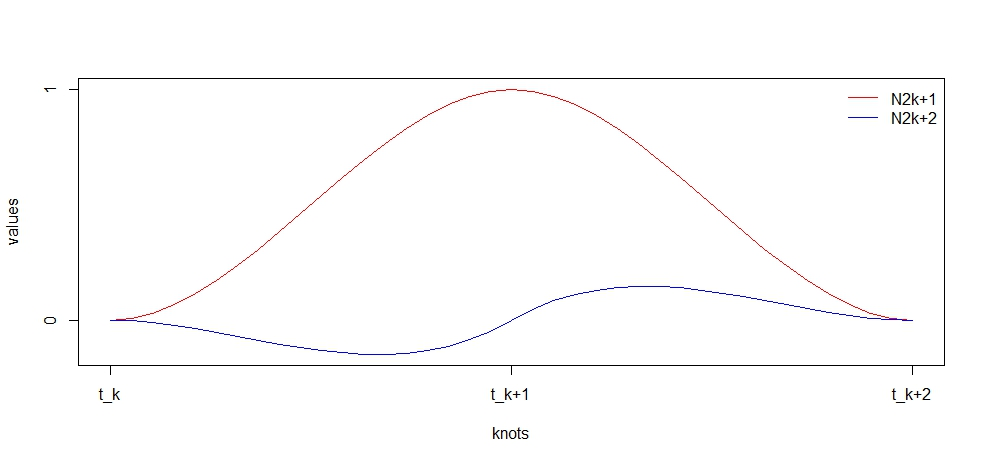
\includegraphics[width=\textwidth, height=9cm]{n2i}
\small \caption{The two basis functions $N_{2k+1}$ and $N_{2k+2}$ on interval $[t_k, t_{k+2}]$. It is apparently that these basis functions are continuous on this interval and have continuous first and second derivatives.}
\end{figure}


As independent basis functions, $N_1(t), \cdots, N_{2n}(t)$ span a $2n$ dimensional space $\mathbb{H}$. For any $f \in \mathbb{H}$, $f$ is represented in the form of
\begin{equation*}
f=\sum_{i=1}^{2n} \theta_i N_i(t).
\end{equation*}

Suppose that we have observations $y_1,\cdots,y_n$ and $v_1,\cdots,v_n$. $f(t)$ can be found by minimizing equation (\ref{mse2}), which reduces to
\begin{equation}
\text{MSE}(\theta, \lambda,\gamma) = (\mathbf{Y}-\mathbf{B}\theta)^T (\mathbf{Y}-\mathbf{B}\theta) +\gamma (\mathbf{V}-\mathbf{C}\theta)^T (\mathbf{V}-\mathbf{C}\theta)+n\lambda \theta^T\Omega\theta
\end{equation}
where $\{\mathbf{B}\}_{ij} = N_j(t_i)$ , $\{\mathbf{C}\}_{ij} = N'_j(t_i)$ and $\{\Omega_{2n} \}_{jk}=\int N''_j(t)N''_k(t)dt$. 
The solution is easily seen to be
\begin{equation}\label{thetahat}
\hat{\theta}=(\mathbf{B}^T\mathbf{B}+\gamma\mathbf{C}^T\mathbf{C}+n\lambda\Omega)^{-1}(\textbf{B}^T\textbf{y}+\gamma\textbf{C}^T\mathbf{V})
\end{equation}
a generalized ridge regression. The fitted smoothing spline is given by
\begin{equation}
\hat{f}(t)=\sum_{i=1}^{2n}N_i(t)\hat{\theta}_i
\end{equation}

A smoothing spline with parameters $\lambda$ and $\gamma$ is an example of a linear smoother \cite{esl2009}. This is because the estimated parameters in (\ref{thetahat}) are a linear combination of the $y_i$ and $v_i$. Denote by $\hat{\mathbf{f}}$ the $2n$ vector of fitted values $\hat{f}(t_i)$ and $\hat{\mathbf{f}'}$ the $2n$ vector of fitted values $\hat{f'}(t_i)$ at the training points $t_i$. Then
\begin{align*}
\hat{\mathbf{f}} &=\mathbf{B}(\mathbf{B}^T\mathbf{B}+\gamma\mathbf{C}^T\mathbf{C}+n\lambda\Omega)^{-1}(\textbf{B}^T\textbf{y}+\gamma\textbf{C}^T\mathbf{V})\\
&=\textbf{S}_{\lambda,\gamma}\textbf{y}+\textbf{T}_{\lambda,\gamma}\textbf{v} \\
\hat{\mathbf{f}'} &=\mathbf{C}(\mathbf{B}^T\mathbf{B}+\gamma\mathbf{C}^T\mathbf{C}+n\lambda\Omega)^{-1}(\textbf{B}^T\textbf{y}+\gamma\textbf{C}^T\mathbf{V})\\
&=\textbf{U}_{\lambda,\gamma}\textbf{y}+\textbf{V}_{\lambda,\gamma}\textbf{v}
\end{align*}
The fitted $\hat{\mathbf{f}}$ and $\hat{\mathbf{f}'}$ are linear in $\mathbf{Y}$ and $\mathbf{V}$, and the finite linear operators $\textbf{S}_{\lambda,\gamma}, \textbf{T}_{\lambda,\gamma}, \textbf{U}_{\lambda,\gamma}$ and $\textbf{V}_{\lambda,\gamma}$ are known as the smoother matrices. One consequence of this linearity is that the recipe for producing $\hat{\mathbf{f}}$ and $\hat{\mathbf{f}'}$ from $\mathbf{Y}$ and $\mathbf{V}$, do not depend on $\mathbf{Y}$ and $\mathbf{V}$ themselves; $\textbf{S}_{\lambda,\gamma}, \textbf{T}_{\lambda,\gamma}, \textbf{U}_{\lambda,\gamma}$ and $\textbf{V}_{\lambda,\gamma}$ depend only on the $t_i,\lambda$ and $\gamma$.

Suppose in a traditional least squares fitting, $\mathbf{B}_\xi$ is $N \times M$ matrix of $M$ cubic-spline basis functions evaluated at the $N$ training points $x_i$, with knot sequence $\xi$ and $M \ll N$. Then the vector of fitted spline values is given by
\begin{align*}
\hat{\mathbf{f}}&=\mathbf{B}_\xi(\mathbf{B}^T_\xi\mathbf{B}_\xi)^{-1}\mathbf{B}_\xi\mathbf{Y}\\
&=\mathbf{H}_\xi\mathbf{Y}
\end{align*}
Here the linear operator $\mathbf{H}_\xi$ is a symmetric, positive semidefinite matrices, and $\mathbf{H}_\xi\mathbf{H}_\xi=\mathbf{H}_\xi$ (idempotent). In our case, it is easily seen that $\textbf{S}_{\lambda,\gamma}, \textbf{T}_{\lambda,\gamma}, \textbf{U}_{\lambda,\gamma}$ and $\textbf{V}_{\lambda,\gamma}$ are symmetric, positive semidefinite matrices as well. However, only when $\lambda=\gamma=0$, the matrix $\textbf{S}_{\lambda=0,\gamma=0}$ is idempotent.


\subsection{Tractor Spline Estimated by GP}

With tractor spline basis functions $N_1(t), \cdots, N_{2n}(t)$, given the sample points $t_i, i=1, \cdots, n$ in space $\mathbb{H}$ and noting that the space
\begin{equation*}
\mathbb{A}=\{f: f=\sum_{i=1}^{n}\alpha_iR(t_i,\cdot) \} 
\end{equation*}
is one linear subspace of $\mathbb{H}$, 
\begin{equation*}
\mathbb{B}=\{f: f=\sum_{i=1}^{n}\beta_i \dot{R}(t_i,\cdot) \} 
\end{equation*}
is another linear subspace of $\mathbb{H}$, where $\dot{R}$ is defined in equation (\ref{dotr}). After calculating, it is proved that $\mathbb{A} \cap \mathbb{B} = \emptyset$. Then $f \in \mathbb{H}$ can be written as
\begin{equation}\label{etaeq}
f(t)=\sum_{i=1}^{n}c_iR(t_i,t)+\sum_{i=1}^{n}d_i \dot{R}(t_i,t)+\rho(t)
\end{equation}
where $c_i, d_i$ are coefficients, $\rho(t) \in \mathbb{H} \ominus (\mathbb{A} \oplus \mathbb{B})$, and 
\begin{equation}\label{etaeq2}
f'(t)=\sum_{i=1}^{n}c_iR'(t_i,t)+\sum_{i=1}^{n}d_i \dot{R}'(t_i,t)+\rho'(t).
\end{equation}

The equation (\ref{mse2}) can be written as
\begin{align*}
&\frac{1}{n}\sum_{i=1}^n (y_i -\sum_{j=1}^{n}c_jR(t_j,t_i)- \sum_{j=1}^{n}d_j\dot{R}(t_j,t_i) -\rho(t_i))^2\\+&
\frac{\gamma}{n}\sum_{i=1}^n (v_i -\sum_{j=1}^{n}c_jR'(t_j,t_i)- \sum_{j=1}^{n}d_j\dot{R}'(t_j,t_i) -\rho'(t_i))^2 \\
+&\lambda \int_{t_1}^{t_n} (\sum_{j=1}^{n}c_jR''(t_j,t)+ \sum_{j=1}^{n}d_j\dot{R}''(t_j,t) +\rho''(t))^2dt
\end{align*}
By orthogonality, $\rho(t_i) = <R(t_i,\cdot),\rho>=0$, %$\rho(t_i) =<\rho,R'(\cdot,t_i)>=<\dot{R}(t_i,\cdot),\rho>=0$, 
and $\rho'(t_i) = <\dot{R}(t_i,\cdot),\rho>=0$, where $i=1,\cdots,n$. 

Denoting by $Q$ the $n \times n$ matrix with the $(i,j)$th entry $R(t_i,t_j)$, by $P$ the $n \times n$ matrix with the $(i,j)$th entry $\dot{R}(t_i,t_j)$ the equation (\ref{mse2}) can be written as
\begin{equation}\label{matrixeq}
(\mathbf{Y}-Q\mathbf{c}-P\mathbf{d})^T(\mathbf{Y}-Q\mathbf{c}-P\mathbf{d})+\gamma (\mathbf{V}-\frac{\partial Q}{\partial t}\mathbf{c}-\frac{\partial P}{\partial t}\mathbf{d})^T(\mathbf{V}-\frac{\partial Q}{\partial t}\mathbf{c}-\frac{\partial P}{\partial t}\mathbf{d})+n\lambda \Omega+\lambda(\rho,\rho).
\end{equation}
Note that $\rho$ only appears in the third term in $(\ref{matrixeq})$, which is minimized at $\rho=0$. Hence, a polynomial smoothing spline resides in the space $\mathbb{A} \oplus \mathbb{B}$ of finite dimension. Then the solution could be computed via minimization of term in $(\ref{matrixeq})$ with respect to $\mathbf{c}$ and $\mathbf{d}$, \cite{gubook}.

\section{Cross Validation}

Probably the simplest and most widely used method for estimating prediction error is cross-validation, \cite{esl2009}. Assuming that the random error has zero mean, the true regression curve $f$ has the property that, if an observation $y$ is taken at a point $t$, the value $f(t)$ is the best predictor of $y$ in terms of mean square error, \cite{green1993nonparametric}. 

Now we focus on an observation $y_i$ at point $t_i$ as being a new observation by omitting it from the set of data, which are used to estimate $\hat{f}$. Denote by $\hat{f}^{(-i)}(t,\lambda)$ the estimated function from the remaining data, where $\lambda$ is the smoothing parameter. Then $\hat{f}^{(-i)}(t,\lambda)$ minimizes 
\begin{align*}
\frac{1}{n}\sum_{j \neq i}(y_j-f(t_j))^2+\lambda \int f''^2dt
\end{align*}
 and $\lambda$ can be quantified by cross-validation score function
\begin{align*}
CV(\lambda)=\frac{1}{n}\sum_{i=1}^{n}\{y_i-\hat{f}^{(-i)}(t_i,\lambda)\}^2.
\end{align*}
The basis idea of cross-validation is to choose the value of $\lambda$ that minimizes $CV(\lambda)$, \cite{green1993nonparametric}.

Generalized Cross-Validation (GCV) is a modified form for choosing smoothing parameters, and the value $\lambda$ can be carried out by minimizing the function 
\begin{align*}
GCV(\lambda)=\frac{1}{n}\frac{\sum_{i=1}^{n}\{y_i-\hat{f}(t_i,\lambda)\}^2}{\{1-\frac{1}{n}tr(A(\lambda))\}^2}.
\end{align*}
For weighted smoothing splines, the residual sum of squares is 
\begin{align*}
\sum_{i=1}^{n}w_i (y_i-f(t_i))^2
\end{align*}
and the cross-validation score function is 
\begin{align*}
CV(\lambda)=\sum_{i=1}^n w_i\{\frac{y_i-\hat{f}(t_i,\lambda)}{(I-A(\lambda))_{ii}}\}^2.
\end{align*}
Then we assume that the cross-validation score function for tractor spline (TCV) is in the form of
\begin{align*}
TCV(\lambda, \gamma)=\frac{1}{n}\frac{\sum |y_i-f(t_i)|^2+\sum \gamma |v_i-f'(t_i)|^2}{|1-\frac{1}{n}tr(\hat{\theta}(\lambda,\gamma))|^2}
\end{align*}

\subsection{Leave-one-out Cross Validation}
As the parameter $\hat{\theta}=(B^TB+\gamma C^TC+n\Omega_\lambda)^{-1}(B^Ty+\gamma C^Tv)$, then
\begin{align*}
 \hat{f}=B\hat{\theta}=B(B^TB+\gamma C^TC+n\Omega_\lambda)^{-1}B^Tx+B(B^TB+\gamma C^TC+n\Omega_\lambda)^{-1}C^Tv=Sy+Tv\\
\hat{f}'=C\hat{\theta}=C(B^TB+\gamma C^TC+n\Omega_\lambda)^{-1}B^Tx+C(B^TB+\gamma C^TC+n\Omega_\lambda)^{-1}C^Tv=Uy+Vv
\end{align*}
Then the cross validation formula could be represented in the form of 
\begin{equation}
CV=\sum \frac{\hat{f}(t_i)-y_i+\gamma \frac{T_{ii}}{1-\gamma V_{ii}}(\hat{f}'(t_i)-v_i)}{1-S_{ii}-\gamma\frac{T_{ii}}{1-\gamma V_{ii}}U_{ii}}
\end{equation}

\subsection{K-Fold Cross Validation}

Based on the procedure given by \cite{wahba1975completely}, we  follow the improved steps to calculate a K-fold cross validation. 

Step 1. Remove the first data $t_1$ and last date $t_n$ from the dataset.

Step 2. Divide dataset into k groups:
\begin{align*}
& \mbox{Group 1}: t_2, t_{2+k}, \cdots \\
& \mbox{Group 2}: t_3, t_{3+k}, \cdots \\
& \vdots \\
& \mbox{Group k}: t_{k+1}, t_{2k+1}, \cdots
\end{align*}

Step 3. Guess values of $\lambda_{down}, \lambda_{up}$ and $\gamma$.

Step 4. Delete the first group of data. Fit a smoothing spline to the first data, the rest groups of dataset and the last data, with  $\lambda_{down}, \lambda_{up}$ and $\gamma$ in step 3. Compute the sum of squared deviations of this smoothing spline from the deleted data points.

Step 5. Delete instead the second group of data. Fit a smoothing spline to the remaining data with  $\lambda_{down}, \lambda_{up}$ and $\gamma$. Compute the sum of squared deviations of the spline from deleted data points.

Step 6. Repeat Step 5 for the 3rd, 4th, $\cdots$, $k$th group of data.

Step 7. Add the sums of squared deviations from steps 4 to 6 and divide by $k$. This is the cross validation score of three parameters  $\lambda_{down}, \lambda_{up}$ and $\gamma$.

Step 8. Vary  $\lambda_{down}, \lambda_{up}$ and $\gamma$ systematically and repeat steps 4-7 until CV shows a minimum.

\clearemptydoublepage

%\setcounter{chapter}{1}
%\include{Chapters/2.Preliminaries/preliminaries_v5}
%\clearemptydoublepage


%\setcounter{chapter}{2}
%\include{Chapters/3.Time-domain_analysis/time_domain_v4}
%\clearemptydoublepage

%\setcounter{chapter}{3}
%\include{Chapters/4.Experiments/experiments_v3}
%\clearemptydoublepage

%\setcounter{chapter}{4}
%\include{Chapters/5.Data_analysis/data_analysis_v3}
%\clearemptydoublepage

%\setcounter{chapter}{5}
%\include{Chapters/6.Natural_modes/natural_modes_v3}
%\clearemptydoublepage

%\setcounter{chapter}{6}
%\include{Chapters/7.Further_modelling/further_modelling_v3}
%\clearemptydoublepage

%\setcounter{chapter}{7}
%\include{Chapters/8.Two_disks/two_disks_v3}
%\clearemptydoublepage

%\setcounter{chapter}{8}
%\include{Chapters/9.Conclusion/concl_v2}
%\clearemptydoublepage

%% Bibliography

\bibliographystyle{otago}
\bibliography{thesis}
\clearemptydoublepage


%% Appendices

\appendix
%\include{Appendices/Edge_conditions/App_edge_cond}
%\clearemptydoublepage


\section*{Penalty Matrix in (\ref{tractormse})}


The $k$-th $\Omega^{(k)}$ is a $2n \times 2n$ matrix in the form of
\begin{align*}
\Omega_{2k-1,2k-1}^{(k)} & =\int_{t_{k}}^{t_{k+1}} \frac{d^2 h_{00}^{(k)}(t)}{dt^2}  \frac{d^2 h_{00}^{(k)}(t)}{dt^2} dt=\frac{12}{\Delta_k^3}\\
\Omega_{2k-1,2k}^{(k)} &=\int_{t_{k}}^{t_{k+1}} \frac{d^2 h_{00}^{(k)}(t)}{dt^2}  \frac{d^2 h_{10}^{(k)}(t)}{dt^2} dt=\frac{6}{\Delta_k^2}\\
\Omega_{2k-1,2k+1}^{(k)} &=\int_{t_{k}}^{t_{k+1}} \frac{d^2 h_{00}^{(k)}(t)}{dt^2}  \frac{d^2 h_{01}^{(k+1)}(t)}{dt^2} dt=\frac{-12}{\Delta_k^3}\\
\Omega_{2k-1,2k+2}^{(k)} &=\int_{t_{k}}^{t_{k+1}} \frac{d^2 h_{00}^{(k)}(t)}{dt^2}  \frac{d^2 h_{11}^{(k+1)}(t)}{dt^2} dt=\frac{6}{\Delta_k^2}\\
\Omega_{2k,2k}^{(k)} &=\int_{t_{k}}^{t_{k+1}} \frac{d^2 h_{10}^{(k)}(t)}{dt^2}  \frac{d^2 h_{10}^{(k)}(t)}{dt^2} dt=\frac{4}{\Delta_k} \\
\Omega_{2k,2k+1}^{(k)} &=\int_{t_{k}}^{t_{k+1}} \frac{d^2 h_{10}^{(k)}(t)}{dt^2}  \frac{d^2 h_{01}^{(k+1)}(t)}{dt^2} dt=\frac{-6}{\Delta_k^2}\\
\Omega_{2k,2k+2}^{(k)} &=\int_{t_{k}}^{t_{k+1}} \frac{d^2 h_{10}^{(k)}(t)}{dt^2}  \frac{d^2 h_{11}^{(k+1)}(t)}{dt^2} dt=\frac{2}{\Delta_k}\\
\Omega_{2k+1,2k+1}^{(k)} &=\int_{t_{k}}^{t_{k+1}} \frac{d^2 h_{01}^{(k+1)}(t)}{dt^2}  \frac{d^2 h_{01}^{(k+1)}(t)}{dt^2} dt=\frac{12}{\Delta_k^3}\\
\Omega_{2k+1,2k+2}^{(k)} &=\int_{t_{k}}^{t_{k+1}} \frac{d^2 h_{01}^{(k+1)}(t)}{dt^2}  \frac{d^2 h_{11}^{(k+1)}(t)}{dt^2} dt=\frac{-6}{\Delta_k^2}\\
\Omega_{2k+2,2k+2}^{(k)} &=\int_{t_{k}}^{t_{k+1}} \frac{d^2 h_{11}^{(k+1)}(t)}{dt^2}  \frac{d^2 h_{11}^{(k+1)}(t)}{dt^2} dt=\frac{4}{\Delta_k}
\end{align*}
$k=1,2,\cdots,n-1$. It's a bandwidth four matrix. Then
\begin{equation*}
\mathbf{\Omega}=\sum_{k=1}^{n-1}\Omega^{(k)}
\end{equation*}



\section*{Penalty Matrix in (\ref{matrixeq})}
The penalty matrix $\Omega$ in (\ref{matrixeq}) is a combination of three sub matrix $\Omega_1$, $\Omega_2$ and $\Omega_3$, which are in the following form

\begin{align*}
\Omega_{k,k}^{(1)} & =\int_{t_{k}}^{t_{k+1}} \frac{d^2 h_{00}^{(k)}(t)}{dt^2}  \frac{d^2 h_{00}^{(k)}(t)}{dt^2} dt=\frac{12}{\Delta_k^3}\\
\Omega_{k,k+1}^{(1)} &=\int_{t_{k}}^{t_{k+1}} \frac{d^2 h_{00}^{(k)}(t)}{dt^2}  \frac{d^2 h_{01}^{(k+1)}(t)}{dt^2} dt=\frac{-12}{\Delta_k^3}\\
\Omega_{k+1,k+1}^{(1)} &=\int_{t_{k}}^{t_{k+1}} \frac{d^2 h_{01}^{(k+1)}(t)}{dt^2}  \frac{d^2 h_{01}^{(k+1)}(t)}{dt^2} dt=\frac{12}{\Delta_k^3}\\
\Omega_{k,k}^{(2)} &=\int_{t_{k}}^{t_{k+1}} \frac{d^2 h_{10}^{(k)}(t)}{dt^2}  \frac{d^2 h_{10}^{(k)}(t)}{dt^2} dt=\frac{4}{\Delta_k} \\
\Omega_{k,k+1}^{(2)} &=\int_{t_{k}}^{t_{k+1}} \frac{d^2 h_{10}^{(k)}(t)}{dt^2}  \frac{d^2 h_{11}^{(k+1)}(t)}{dt^2} dt=\frac{2}{\Delta_k}\\
\Omega_{k+1,k+1}^{(2)} &=\int_{t_{k}}^{t_{k+1}} \frac{d^2 h_{11}^{(k+1)}(t)}{dt^2}  \frac{d^2 h_{11}^{(k+1)}(t)}{dt^2} dt=\frac{4}{\Delta_k}\\
\Omega_{k,k}^{(3)} &=\int_{t_{k}}^{t_{k+1}} \frac{d^2 h_{00}^{(k)}(t)}{dt^2}  \frac{d^2 h_{10}^{(k)}(t)}{dt^2} dt=\frac{6}{\Delta_k^2}\\
\Omega_{k,k+1}^{(3)} &=\int_{t_{k}}^{t_{k+1}} \frac{d^2 h_{00}^{(k)}(t)}{dt^2}  \frac{d^2 h_{11}^{(k+1)}(t)}{dt^2} dt=\frac{6}{\Delta_k^2}\\
\Omega_{k+1,k}^{(3)} &=\int_{t_{k}}^{t_{k+1}} \frac{d^2 h_{10}^{(k)}(t)}{dt^2}  \frac{d^2 h_{01}^{(k+1)}(t)}{dt^2} dt=\frac{-6}{\Delta_k^2}\\
\Omega_{k+1,k+1}^{(3)} &=\int_{t_{k}}^{t_{k+1}} \frac{d^2 h_{01}^{(k+1)}(t)}{dt^2}  \frac{d^2 h_{11}^{(k+1)}(t)}{dt^2} dt=\frac{-6}{\Delta_k^2}
\end{align*}


\section*{Proof of Theorem \ref{basisindependent}}

\begin{proof}
It is obviously that every basis functions are continuous on subinterval $[t_k,t_{k+1}]$. We firstly prove that these basis functions are independent. 

We have $2n$ basis functions and $n$ knots. Then choose $t_1, \frac{t_1+t_2}{2}, t_2, \frac{t_2+t_3}{2}, \cdots, t_{n-1}, \frac{t_{n-1}+t_n}{3}$, $\frac{2(t_{n-1}+t_n)}{3}, t_n$ as new $2n$ knots, and denoted by $c_1,c_2,\cdots,c_{2n}$. Then the determinant is
\begin{equation}\label{matrixD}
D(c_1,c_2,\cdots,c_{2n})=
\begin{vmatrix}
N_1(c_1) & N_1(c_2) & \cdots& N_1(c_{2n})\\
N_2(c_1) & N_2(c_2)& \cdots & N_2(c_{2n})\\
 \vdots  &  \vdots  & \ddots  & \vdots  \\  
N_{2n}(c_1) & N_{2n}(c_2) & \cdots & N_{2n}(c_{2n})\\
\end{vmatrix}
=
\begin{vmatrix}
1 & a_{12} & 0 & 0 & \cdots& 0 & 0 \\
0 & a_{22} & 0 & 0 & \cdots& 0 & 0\\
0 & a_{32} & 1 & a_{34} & \cdots& 0 & 0\\
 \vdots  &  \vdots  &  \vdots &  \vdots & \ddots  & \vdots   &  \vdots\\  
0 & 0 & 0 & 0 & \cdots& a_{2n-1,2n-1} & 1\\
0 & 0 & 0 & 0 & \cdots& a_{2n,2n-1} & 0 \\
\end{vmatrix},
\end{equation}
where $D(c_1,c_2,\cdots,c_{2n})=\begin{cases}
N_1(t_1)=1 \\
N_1(\frac{t_1+t_2}{2})=a_{12} \\
N_2(t_1)=0 \\
N_2(\frac{t_1+t_2}{2})=a_{22} \\
N_{2k+1}(\frac{t_k+t_{k+1}}{2})=a_{2k+1,2k} & k=1,2,\cdots,2n \\ 
N_{2k+1}(t_{k+1})=1 & k=1,2,\cdots,2n \\ 
N_{2k+1}(\frac{t_{k+1}+t_{k+2}}{2})=a_{2k+1,2k+2} & k=1,2,\cdots,2n \\ 
N_{2k+2}(\frac{t_k+t_{k+1}}{2})=a_{2k+2,2k} & k=1,2,\cdots,2n \\ 
N_{2k+2}(\frac{t_{k+1}+t_{k+2}}{2})=a_{2k+2,2k+2}  & k=1,2,\cdots,2n\\ 
N_{2n-1}(t_{2n-1})=0 \\
N_{2n-1}(\frac{t_{2n-1}+t_{2n}}{3})=a_{2n-1,2n-2} \\
N_{2n-1}(\frac{2(t_{2n-1}+t_{2n})}{3})=a_{2n-1,2n-1} \\
N_{2n-1}(t_{2n})=1 \\
N_{2n}(\frac{t_{2n-1}+t_{2n}}{3})=a_{2n,2n-2} \\
N_{2n}(\frac{2(t_{2n-1}+t_{2n})}{3})=a_{2n,2n-1} \\
N_{2n}(t_{2n})=0 \\
0 &  otherwise
\end{cases}$,\\
and $a_{ij}\neq 0.$ After decomposing determinant $D$ in equation (\ref{matrixD}),  gives
\begin{align*}
\det D= & 
\begin{vmatrix}
 a_{22} & 0 & 0 & \cdots& 0 & 0\\
 a_{32} & 1 & a_{34} & \cdots& 0 & 0\\
  \vdots  &  \vdots &  \vdots & \ddots  & \vdots   &  \vdots\\  
0 & 0 & 0 & \cdots& a_{2n-1,2n-1} & 1\\
0 & 0 & 0 & \cdots& a_{2n,2n-1} & 0 \\
\end{vmatrix}
=a_{22}
\begin{vmatrix}
 1 & a_{34} & \cdots& 0 & 0\\
  \vdots &  \vdots & \ddots  & \vdots   &  \vdots\\  
 0 & 0 & \cdots& a_{2n-1,2n-1} & 1\\
 0 & 0 & \cdots& a_{2n,2n-1} & 0 \\
\end{vmatrix}\\
=& \cdots =a_{22}a_{44}\cdots a_{2n-4,2n-4} 
\begin{vmatrix}
a_{2n-2,2n-2} & a_{2n-2,2n-1}  & 0\\
a_{2n-1,2n-2} & a_{2n-1,2n-1} & 1\\
 a_{2n,2n-2} &  a_{2n,2n-1} & 0 \\
\end{vmatrix}\\
=& a_{22}a_{44}\cdots a_{2n-4,2n-4} (a_{2n-2,2n-1}a_{2n,2n-2}-a_{2n,2n-1}a_{2n-2,2n-2}) \neq 0.
\end{align*}
With the conclusion in Lemma 1, $N_1(t),\ldots,N_{2n}(t)$  are linearly independent on interval $[t_1, t_n]$.

Secondly, we prove that basis functions represent any cubic function on each interval $[t_k, t_{k+1}]$. Due to the definition of cubic spline, on interval $[t_k, t_{k+1}]$, a cubic spline $g(t)$ can be written in the form of
\begin{eqnarray}
g(t)=d_k (t-t_k)^3+c_k(t-t_k)^2+b_k(t-t_k)+a_k, \mbox{for $t_k \leq t \leq t_{k+1}$}
\end{eqnarray}
For any $f(t)$ on $[t_1, t_n]$, it can be represented as $f(t)=\sum_{k=1}^{2n} \theta_k N_k(t)$. Then for $\forall t \in [t_k,t_{k+1}]$, we have
\begin{align*}
f(t)=\begin{cases}
\theta_{2k-1}N_{2k-1}(t)+\theta_{2k}N_{2k}(t)+\theta_{2k+1}N_{2k+1}(t)+\theta_{2k+2}N_{2k+3}(t), & t_k \leq t \leq t_{k+1}  \\
0, & \mbox{otherwise}\\
\end{cases},
\end{align*}
thus
\begin{align*}
f(t)=&\theta_{2k-1}\{ 2(\frac{t-t_{k}}{t_{k+1}-t_{k}})^3-3(\frac{t-t_{k}}{t_{k+1}-t_{k}})^2+1  \} +\theta_{2k} \{  \frac{(t-t_{k})^3}{(t_{k+1}-t_{k})^2}-2\frac{(t-t_{k})^2}{t_{k+1}-t_{k}}+(t-t_{k}) \} \\
+&\theta_{2k+1} \{ -2(\frac{t-t_k}{t_{k+1}-t_k})^3+3(\frac{t-t_k}{t_{k+1}-t_k})^2  \}  +\theta_{2k+2} \{  \frac{(t-t_k)^3}{(t_{k+1}-t_k)^2}-\frac{(t-t_k)^2}{t_{k+1}-t_k} \}.
\end{align*}
After rearranging, we have
\begin{align*}
f(t)=& \{ \frac{2\theta_{2k-1}}{(t_{k+1}-t_{k})^3} +\frac{\theta_{2k}}{(t_{k+1}-t_{k})^2} -\frac{2\theta_{2k+1}}{(t_{k+1}-t_{k})^3} +\frac{\theta_{2k+2}}{(t_{k+1}-t_{k})^2} \} (t-t_k)^3 \\
+&  \{ -\frac{3\theta_{2k-1}}{(t_{k+1}-t_{k})^2} -\frac{2\theta_{2k}}{(t_{k+1}-t_{k})} +\frac{3\theta_{2k+1}}{(t_{k+1}-t_{k})^2} - \frac{\theta_{2k+2}}{(t_{k+1}-t_{k})} \} (t-t_k)^2 \\
+&  \theta_{2k} (t-t_k) +\theta_{2k-1}
\end{align*}
where coefficients are
\begin{align*}
\begin{cases}
\theta_{2k-1}=a_k\\
\theta_{2k}=b_k\\
-\frac{3\theta_{2k-1}}{(t_{k+1}-t_{k})^2} -\frac{2\theta_{2k}}{(t_{k+1}-t_{k})} +\frac{3\theta_{2k+1}}{(t_{k+1}-t_{k})^2} - \frac{\theta_{2k+2}}{(t_{k+1}-t_{k})}=c_k\\
\frac{2\theta_{2k-1}}{(t_{k+1}-t_{k})^3} +\frac{\theta_{2k}}{(t_{k+1}-t_{k})^2} -\frac{2\theta_{2k+1}}{(t_{k+1}-t_{k})^3} +\frac{\theta_{2k+2}}{(t_{k+1}-t_{k})^2}=d_k
\end{cases}
\end{align*}
the resulting can always be solved for $\theta_{2k-1}, \theta_{2k},\theta_{2k+1},\theta_{2k+2}$ in terms of $a_k,b_k,c_k,d_k$ on interval $[t_k, t_{k+1}]$. So cubic spline on each interval can be represented by basis functions. 

Finally, we will prove basis functions are continuous on $[t_1, t_n]$. For any knot $t_k$, where $t_1< t_k <t_n$, it is known that $f(t_k)=\theta_{2k-1}$. Moreover, 
\begin{align*}
\lim\limits_{t\rightarrow t_k+} f(t) = \lim\limits_{t\rightarrow t_k+} (\theta_{2k-1}N_{2k-1}(t)+\theta_{2k}N_{2k}(t)+\theta_{2k+1}N_{2k+1}(t)+\theta_{2k+2}N_{2k+3}(t))=\theta_{2k-1},\\
\lim\limits_{t\rightarrow t_k-} f(t) = \lim\limits_{t\rightarrow t_k-} (\theta_{2k-1}N_{2k-1}(t)+\theta_{2k}N_{2k}(t)+\theta_{2k+1}N_{2k+1}(t)+\theta_{2k+2}N_{2k+3}(t))=\theta_{2k-1}.
\end{align*}
So
\begin{align*}
\lim\limits_{t\rightarrow t_k+} f(t) =\lim\limits_{t\rightarrow t_k-} f(t) =f(t),
\end{align*}
$f(t)$ is continuous at knots, and then continuous on whole interval $[t_1,t_n]$.

$f(t)$ is a continuous cubic spline on interval $[t_1,t_n]$, then $f(t)$ has continuous first and second derivatives.
\end{proof}


\section*{Proof of Lemma \ref{cvlemma}}

\begin{proof}
For any spline $f$, 
\begin{equation}
\begin{split}
&\frac{1}{n}\sum_{j=1}^{n}(y_j^*-f(t_j))^2+\frac{\gamma}{n} \sum_{j=1}^{n}(v_j^*-f'(t_j))+\lambda\int f''^2 \\
\geq&\frac{1}{n}\sum_{j\neq i}^{n}(y_j^*-f(t_j))^2+\frac{\gamma}{n} \sum_{j\neq i}^{n}(v_j^*-f'(t_j))+\lambda\int f''^2\\
\geq&\frac{1}{n}\sum_{j\neq i}^{n}(y_j^*-\hat{f}^{(-i)}(t_j))^2+\frac{\gamma}{n} \sum_{j\neq i}^{n}(v_j^*-\hat{f}'^{(-i)}(t_j))+\lambda\int \hat{f}^{(-i)''2}\\
=&\frac{1}{n}\sum_{j=1}^{n}(y_j^*-\hat{f}^{(-i)}(t_j))^2+\frac{\gamma}{n} \sum_{j=1}^{n}(v_j^*-\hat{f}'^{(-i)}(t_j))+\lambda\int \hat{f}^{(-i)''2}
\end{split}
\end{equation}
by the definition of $\hat{f}^{(-i)}$, $\hat{f}'^{(-i)}$ and $y_i^*=\hat{f}^{(-i)}(t_i)$, $v_i^*=\hat{f}'^{(-i)}(t_i)$. It follows that $\hat{f}^{(-i)}$ is the minimizer of the MSE function (\ref{mse2}), so that
\begin{align}
\mathbf{\hat{f}}^{(-i)}&=S\mathbf{y}^*+\gamma T\mathbf{v}^*\\
\mathbf{\hat{f}}'^{(-i)}&=U\mathbf{y}^*+\gamma V\mathbf{v}^*
\end{align}
\end{proof}


\section*{Proof of Theorem \ref{cvscore}}

\begin{proof}
\begin{equation}\label{th3proofeq1}
\begin{split}
\hat{f}^{(-i)}(t_i)-y_i=& \sum_{j=1}^{n}S_{ij}y_j^*+ \gamma \sum_{j=1}^{n}T_{ij}v_j^*-y_i^*\\
=&\sum_{j\neq i}^{n}S_{ij}y_j+ \gamma \sum_{j\neq i}^{n}T_{ij}v_j+S_{ii}\hat{f}^{(-i)}(t_i)+\gamma T_{ii}\hat{f}'^{(-i)}(t_i)-y_i\\
=&\sum_{j=1}^{n}S_{ij}y_j+ \gamma \sum_{j=1}^{n}T_{ij}v_j+S_{ii}(\hat{f}^{(-i)}(t_i)-y_i)+\gamma T_{ii}(\hat{f}'^{(-i)}(t_i)-v_i)-y_i\\
=&(\hat{f}(t_i)-y_i)+S_{ii}(\hat{f}^{(-i)}(t_i)-y_i)+\gamma T_{ii}(\hat{f}'^{(-i)}(t_i)-v_i).
\end{split}
\end{equation}
Additionally, 
\begin{equation}
\begin{split}
\hat{f}'^{(-i)}(t_i)-v_i=& \sum_{j=1}^{n}U_{ij}y_j^*+ \gamma \sum_{j=1}^{n}V_{ij}v_j^*-v_i^*\\
=&\sum_{j\neq i}^{n}U_{ij}y_j+ \gamma \sum_{j\neq i}^{n}V_{ij}v_j+U_{ii}\hat{f}^{(-i)}(t_i)+\gamma V_{ii}\hat{f}'^{(-i)}(t_i)-v_i\\
=&\sum_{j=1}^{n}U_{ij}y_j+ \gamma \sum_{j=1}^{n}V_{ij}v_j+U_{ii}(\hat{f}^{(-i)}(t_i)-y_i)+\gamma V_{ii}(\hat{f}'^{(-i)}(t_i)-v_i)-v_i\\
=&(\hat{f}'(t_i)-v_i)+U_{ii}(\hat{f}^{(-i)}(t_i)-y_i)+\gamma V_{ii}(\hat{f}'^{(-i)}(t_i)-v_i).
\end{split}
\end{equation}
Then
\begin{equation}\label{th3proofeq2}
\hat{f}'^{(-i)}(t_i)-v_i = \frac{\hat{f}'(t_i)-v_i}{1-\gamma V_{ii}}+ \frac{U_{ii}(\hat{f}^{(-i)}(t_i)-y_i)}{1-\gamma V_{ii}}.
\end{equation}
After substituting equation (\ref{th3proofeq2}) into (\ref{th3proofeq1}), we get
\begin{equation}
\hat{f}^{(-i)}(t_i)-y_i=\frac{\hat{f}(t_i)-y_i+\gamma \frac{T_{ii}}{1-\gamma V_{ii}}(\hat{f}'(t_i)-v_i)}{1-S_{ii}-\gamma\frac{T_{ii}}{1-\gamma V_{ii}}U_{ii}}.
\end{equation}
Then
\begin{equation}
CV(\lambda,\gamma)=\frac{1}{n}\sum_{i=1}^{n}\frac{\hat{f}(t_i)-y_i+\gamma \frac{T_{ii}}{1-\gamma V_{ii}}(\hat{f}'(t_i)-v_i)}{1-S_{ii}-\gamma\frac{T_{ii}}{1-\gamma V_{ii}}U_{ii}}.
\end{equation}
\end{proof}

\clearemptydoublepage

%\include{Appendices/Fourier_inversion/fourier}
%\clearemptydoublepage

%\include{Appendices/Pointwise_comparison/comparison}
%\clearemptydoublepage

%\include{Appendices/Natural_modes_norm/norm}
%\clearemptydoublepage

%\include{Appendices/Natural_frequencies/nat_freq}

\end{document}


\end{document}  